\documentclass[10pt,twocolumn]{article}

\usepackage[letterpaper,margin=0.68in,top=0.72in,bottom=0.72in]{geometry}
\usepackage[T1]{fontenc}
\usepackage{lmodern}
\usepackage{microtype}
\usepackage{amsmath,amssymb,mathtools}
\usepackage{booktabs,tabularx,array,multirow}
\usepackage{graphicx}
\usepackage{xcolor}
\usepackage{tikz}
\usetikzlibrary{positioning,arrows.meta,fit,calc}
\usepackage{enumitem}
\usepackage{balance}
\usepackage[backend=biber,style=ieee,sorting=none,doi=true,url=true,isbn=false]{biblatex}
\usepackage{placeins}
\usepackage{url}
\usepackage[hidelinks]{hyperref}
\hypersetup{
  pdftitle={Qoralis Engine: A System Characterization of Sparse-Expert Inference Across GPU, RAM, and NVMe Tiers},
  pdfauthor={Qoralis Engine Contributors},
  pdfsubject={Implementation and evidence review of the Qoralis v2.1.0 downstream distribution},
  pdfkeywords={mixture of experts, sparse inference, expert offloading, heterogeneous memory, NVMe, GPU inference, reproducibility}
}
\usepackage{fancyhdr}
\usepackage{titlesec}
\addbibresource{references.bib}

\setlength{\columnsep}{0.24in}
\setlength{\parindent}{1em}
\setlength{\parskip}{0pt}
\setlist{nosep,leftmargin=*}
\titleformat{\section}{\bfseries\large}{\thesection.}{0.45em}{}
\titleformat{\subsection}{\bfseries\normalsize}{\thesubsection}{0.4em}{}
\titlespacing*{\section}{0pt}{1.1ex plus .3ex minus .2ex}{.55ex}
\titlespacing*{\subsection}{0pt}{.85ex plus .25ex minus .15ex}{.35ex}
\pagestyle{fancy}
\fancyhf{}
\fancyhead[L]{\small Qoralis Engine: System Characterization}
\fancyhead[R]{\small Technical research report}
\fancyfoot[C]{\small \thepage}
\renewcommand{\headrulewidth}{0.3pt}
\emergencystretch=2em

\newcommand{\qoralis}{\textsc{Qoralis Engine}}
\newcommand{\colibri}{\textsc{Colibri}}
\newcommand{\eg}{e.g.,}
\newcommand{\ie}{i.e.,}
\newcommand{\code}[1]{\texttt{\small\detokenize{#1}}}
\newcommand{\GB}{\,GB}
\newcommand{\tok}{\,token/s}

\title{\vspace{-1.5em}\textbf{Qoralis Engine: A System Characterization of Sparse-Expert Inference Across GPU, RAM, and NVMe Tiers}\\[0.4em]
\large An implementation and evidence review of the Qoralis v2.1.0 downstream distribution}
\author{Qoralis Engine Contributors\\[-0.1em]
\small Independent systems report\\[-0.1em]
\small \url{https://github.com/anku0669/qoralis-engine}}
\date{3 November 2026}

\begin{document}
\twocolumn[\maketitle
\begin{abstract}
Sparse mixture-of-experts (MoE) networks separate parameter capacity from per-token computation: a model may contain hundreds of billions of parameters while activating only a comparatively small expert subset for each token. This sparsity creates an opportunity to place rarely used weights outside accelerator memory, but it also makes inference sensitive to expert locality, storage latency, cache capacity, and the ability to overlap data movement with computation. This paper characterizes \qoralis, a local inference distribution whose v2.1.0 repository contains a family of C inference engines, a Python control plane, hardware-aware resource planning, disk-backed expert access, adaptive expert residency, accelerator backends, and local service interfaces. We describe the three-tier placement model (GPU memory, host RAM, and local storage), the request-to-expert execution path, model-format support, setup and serving surfaces, and the repository's testing and measurement conventions. We relate the design to prior work on sparse MoE, expert offloading, heterogeneous-memory inference, KV-cache management, and speculative decoding. The evaluation is deliberately documentary: performance values are transcribed from the repository's benchmark records and are not claimed as experiments newly run for this paper. Those records illustrate both the feasibility of running very large sparse models under constrained memory and the severe cold-cache cost of storage-bound decoding. Crucially, the repository identifies \qoralis as a downstream distribution of \colibri, originally created by Vincenzo Fornaro; inherited engine algorithms and benchmark records are attributed accordingly. The paper's contribution is a reproducible system map, a critical reading of available evidence, and a concrete evaluation protocol rather than a claim of new model architecture or independently validated speedups.
\end{abstract}
\vspace{0.6em}
\noindent\textbf{Keywords---} mixture of experts, sparse inference, expert offloading, heterogeneous memory, NVMe, GPU inference, model serving, GGUF, reproducibility, local AI.
\vspace{1.0em}
]

\section{Introduction}
The capacity of a neural network is often discussed in terms of total parameters. For sparse MoE models, that number is not the same as the amount of work performed for each token. A router selects a subset of feed-forward experts, and the selected expert outputs are combined into the layer result. Conditional computation makes very large parameter counts practical, but does not make the weights disappear: they still have to be stored, located, and moved to the processor that executes them \cite{shazeer2017,fedus2022,lepikhin2021}.

This mismatch between total model size and active working set is the systems problem addressed by expert offloading. If the dense trunk and a subset of frequently selected experts fit in fast memory, less frequently selected experts can remain in host memory or on local solid-state storage. An inference system can then trade latency for capacity. The trade is highly workload-dependent: expert activation is not uniform, cache warmth changes the number of bytes read per token, and a GPU is beneficial only when transfer and launch costs are repaid by the computation it accelerates. Prior systems have explored GPU/CPU expert placement, prediction, prefetch, and more general GPU/CPU/disk scheduling \cite{xue2024,sheng2023,song2024}.

\qoralis provides a concrete software system for this design space. Its repository describes per-family native C engines, Python setup and orchestration utilities, expert-history tracking, an adaptive cache, an optional GPU expert tier, and APIs for local applications. It supports CPU execution and, where the relevant build and hardware paths are available, Vulkan, CUDA, Metal, and HIP-related backends. It also exposes model selection, import, diagnostics, monitoring, and an OpenAI-compatible serving surface \cite{qoralisrepo,qoralisreadme}.

This work has three goals. First, it explains how the repository's components fit together, rather than presenting a feature checklist. Second, it separates implementation facts from empirical claims and describes what the published benchmark records do and do not establish. Third, it places the system in the research context of MoE serving and heterogeneous-memory inference.

\subsection{Scope and attribution}
The repository's own \code{UPSTREAM.md} states that Qoralis is a downstream distribution of \colibri, originally created by Vincenzo Fornaro (JustVugg). It says the downstream work changes branding, packaging, documentation, launch aliases, and selected interface assets while retaining upstream attribution, Apache-2.0 notices, and the legacy \code{colibri} import namespace and \code{coli} command for compatibility \cite{upstreamnotice,upstreamrepo}. Accordingly, this paper does not claim that the sparse-expert execution algorithms, cache policy, kernels, benchmark results, or model-family implementations originated with the Qoralis rebrand. The technical characterization covers the source tree as distributed under Qoralis v2.1.0; where the repository's performance records originate upstream or from community reports, they are labelled as such.

\subsection{Research questions}
We organize the audit around four questions:
\begin{itemize}
  \item \textbf{RQ1:} How does the engine map a sparse expert working set onto GPU memory, host RAM, and local storage?
  \item \textbf{RQ2:} Which software components coordinate hardware discovery, model admission, expert loading, execution, and serving?
  \item \textbf{RQ3:} What evidence does the repository provide about throughput, expert-cache behavior, correctness, and measurement reproducibility?
  \item \textbf{RQ4:} Which limitations and operational risks remain for users deploying large local models?
\end{itemize}

\section{Background and related work}
\subsection{Sparse MoE inference}
The sparsely gated MoE layer introduced by Shazeer et al. uses a gating network to select a small group of expert subnetworks for an input \cite{shazeer2017}. Subsequent work, including GShard and Switch Transformers, showed how sparsity can scale model capacity while controlling active computation and communication \cite{lepikhin2021,fedus2022}. More recent MoE language models combine this routing structure with model-specific attention, normalization, expert packing, and quantization designs \cite{deepseekv2}.

At inference time, the selected experts are known only after router evaluation. A system must therefore choose between keeping experts resident, predicting or prefetching likely experts, or paying the cost of loading them after a route decision. A disk-backed design also must handle many small or random expert reads, not simply optimize sequential checkpoint loading.

\subsection{Expert offloading and heterogeneous memory}
MoE-Infinity uses activation traces and expert prefetching/caching to reduce host-to-GPU transfer costs for sparse models \cite{xue2024}. PowerInfer exploits nonuniform neuron activations, retaining hot neurons on a consumer GPU and computing colder activations on the CPU \cite{song2024}. FlexGen treats GPU, CPU, and disk as a combined memory/computation system and searches for tensor placement schedules, particularly for throughput-oriented batched generation \cite{sheng2023}. These systems address related but non-identical workloads and scheduling units.

\qoralis operates at expert granularity and explicitly exposes a cold local-storage tier. Its documented runtime uses a per-layer adaptive cache, optional pinned expert histories, a loader pool, and optional lookahead prefetch. Its design objective is primarily to make a large sparse model executable on the host's available memory hierarchy, with accelerator tiers used where they are profitable. This is conceptually close to expert offloading, but this paper does not assert superiority over MoE-Infinity, PowerInfer, or FlexGen: no common, independently reproduced cross-system benchmark is supplied by the audited repository.

\subsection{Serving and decoding optimizations}
PagedAttention and vLLM address a different bottleneck: efficient allocation and sharing of the per-request KV cache during concurrent serving \cite{kwon2023}. Speculative decoding reduces serial target-model decode steps by drafting candidate tokens and verifying them in parallel, while preserving the target distribution under the algorithm's assumptions \cite{leviathan2023}. Qoralis includes model-specific multi-token prediction (MTP) or draft heads where available, but those model-specific implementations should not be conflated with a universal speculative-decoding algorithm or assumed to accelerate every engine. The repository itself documents cases where speculation is disabled because it does not pay \cite{qoralistuning}.


\subsection{Positioning relative to adjacent systems}
The systems below are related in the memory or serving problem they address, but their objectives and scheduling units differ. This distinction matters when interpreting benchmark claims.
\begin{table*}[t]
\centering
\caption{High-level comparison of problem focus. This is a literature-positioning summary, not a feature-by-feature benchmark.}
\label{tab:related}
\scriptsize
\setlength{\tabcolsep}{4pt}
\renewcommand{\arraystretch}{1.12}
\begin{tabularx}{\textwidth}{@{}p{0.18\textwidth}p{0.22\textwidth}p{0.25\textwidth}X@{}}
\toprule
\textbf{System / work} & \textbf{Primary unit} & \textbf{Memory or locality idea} & \textbf{Relation to this paper's system characterization}\\
\midrule
MoE-Infinity \cite{xue2024} & MoE expert activations, sequence/request traces & Activation-aware expert caching and prefetch between host and GPU memory & Closest conceptual comparison for trace-informed expert offload; its published evaluations are not directly comparable to repository records.\\
PowerInfer \cite{song2024} & Neuron activation sparsity & Keep hot neurons on GPU and execute colder activations on CPU & Related heterogeneous execution using activation locality, but at neuron rather than Qoralis's documented expert-store granularity.\\
FlexGen \cite{sheng2023} & Tensor/model layers and batches & Schedule tensors across GPU, CPU, and disk for throughput under constrained accelerator memory & Related three-level memory hierarchy; its workload and optimization objective emphasize high-throughput batched generation.\\
PagedAttention / vLLM \cite{kwon2023} & KV-cache blocks and requests & Page-like KV allocation and sharing to reduce fragmentation and duplication & Addresses serving-state memory rather than offloading routed model experts; complementary rather than equivalent.\\
Qoralis / Colibri lineage \cite{qoralisrepo,upstreamnotice} & Routed experts plus model-family-specific execution state & Per-layer adaptive host cache, pinned usage history, optional GPU expert tier, and local-storage fallback & Focuses on making large sparse checkpoints executable with an explicit local storage tier; evidence reviewed here is repository-reported.\\
\bottomrule
\end{tabularx}
\end{table*}

\subsection{Model interchange and accelerator APIs}
GGUF is an extensible binary format for model files used by GGML-based executors; it carries tensor data and metadata intended to support portable inference loading \cite{ggufspec}. Qoralis documents direct GGUF reading for a range of model families and block quantization formats, alongside checkpoint-specific conversion or preparation paths \cite{qoralisgguf}. CUDA, Vulkan, Metal, and HIP provide distinct execution and memory-management models; backend-specific synchronization, driver, and device behavior must therefore be tested rather than inferred from a shared API surface \cite{cudaguide,vulkanspec}.

\section{System overview}
\subsection{Software components}
The repository is organized around native inference executables and a Python control plane. The C layer contains one principal engine source per model family over shared tensor, quantization, expert, attention, and backend components. The Python layer includes hardware probing, a family registry, model inventory and resource planning, build selection, download/setup orchestration, a CLI launcher, an API gateway, and an MCP server. The Python package requires Python 3.10 or later; conversion, oracle, benchmark, and vision dependencies are optional extras rather than requirements for the native inference core \cite{qoralispyproject,qoralisrepo}.

\begin{figure*}[t]
\centering
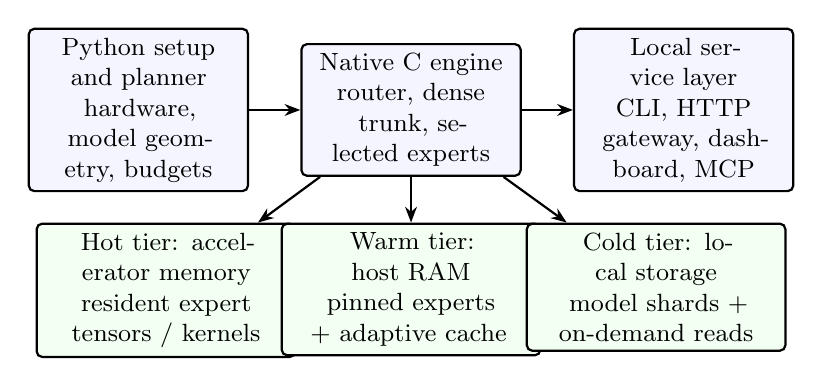
\begin{tikzpicture}[
  node distance=0.42cm and 0.65cm,
  block/.style={draw,rounded corners=2pt,thick,align=center,minimum height=0.72cm,text width=2.55cm,font=\small,fill=blue!4},
  tier/.style={draw,rounded corners=2pt,thick,align=center,minimum height=0.82cm,text width=3.05cm,font=\small,fill=green!5},
  flow/.style={-{Stealth[length=2mm]},thick},
]
\node[block] (setup) {Python setup and planner\\hardware, model geometry, budgets};
\node[block,right=of setup] (engine) {Native C engine\\router, dense trunk, selected experts};
\node[block,right=of engine] (api) {Local service layer\\CLI, HTTP gateway, dashboard, MCP};
\node[tier,below left=0.58cm and 0.05cm of engine] (gpu) {Hot tier: accelerator memory\\resident expert tensors / kernels};
\node[tier,below=0.58cm of engine] (ram) {Warm tier: host RAM\\pinned experts + adaptive cache};
\node[tier,below right=0.58cm and 0.05cm of engine] (ssd) {Cold tier: local storage\\model shards + on-demand reads};
\draw[flow] (setup) -- (engine);
\draw[flow] (engine) -- (api);
\draw[flow] (engine) -- (gpu);
\draw[flow] (engine) -- (ram);
\draw[flow] (engine) -- (ssd);
\end{tikzpicture}
\caption{Conceptual architecture reconstructed from the repository. The Python control plane admits and configures a workload; the C engine routes tokens and obtains experts from a hierarchy of accelerator memory, host RAM, and local storage. Arrows indicate conceptual data and control relationships. Tier-promotion paths are omitted for legibility; not every model/backend uses every tier simultaneously.}
\label{fig:architecture}
\end{figure*}

\subsection{Setup and resource admission}
The one-step setup follows an idempotent sequence: detect hardware, recommend a model that fits, build or obtain a compatible engine, download or resume the model files, configure the runtime, and start the local service. The repository documents that setup does not silently install system packages; it reports the package command that would be needed and lets the user decide whether to run it \cite{qoralisquickstart,qoralissetup}.

Hardware detection collects available RAM, free space at the target model directory, CPU feature flags, and GPU information. The Vulkan path probes devices through the loader when possible and can inspect device-local memory budget; NVIDIA devices are discovered through vendor utilities. The planner also accounts for container memory constraints on supported Linux systems. The intended model-admission rule is not simply that the checkpoint download fits on disk: dense/resident weights, a minimum expert cache, execution workspace, and context state must fit the relevant memory budget \cite{qoralishw,qoralisresource}.

This is important because a 400-GB checkpoint can be operationally possible on a machine with far less than 400 GB of RAM if only its dense trunk and a bounded working set must stay resident. It is not a guarantee of interactive latency. Admission answers whether a model can run under a memory policy; performance depends on the active expert miss rate, storage latency, CPU/GPU throughput, and the prompt and decode workload.

\subsection{Expert placement and runtime path}
The repository describes a five-stage token path: route, union, place, overlap, and learn \cite{qoralisreadme}. For a token at a given layer, the router chooses expert IDs and gates. The implementation can batch/union work across positions so an expert needed by several rows is loaded and computed once for that batch. The placement mechanism checks whether an expert is resident in a faster tier; on a miss, a loader reads it from the backing model files and the runtime schedules the resulting compute.

The expert-store interface in \code{c/expert_store.h} keys an expert by layer and expert index and returns tensor views for gate, up, and down projections. A successful lookup creates a lease that must be released exactly once. Its statistics structure records requests, hits, misses, prefetch activity, bytes read, resident bytes, and capacity bytes. Prefetch is advisory and must not evict an expert with an active lease. This contract makes tensor lifetime and eviction behavior explicit at the shared interface \cite{qoralisexpertstore}.

The repository documents a per-layer adaptive cache plus a pinned set learned from router-usage history. The history is written to a local usage file, and the ranking can be adapted with decay so older usage does not dominate a changed workload. The purpose is placement, not routing: a placement history changes where weights are found, not the router logits or expert IDs. Explicit quality-affecting options, including adaptive expert top-p/top-k variants, are separate opt-ins and are reported as such in the tuning documentation \cite{qoralisroute,qoralistuning}.

\subsection{Three-tier memory model}
Let $E_l$ be the experts in layer $l$, $R_{l,t}\subseteq E_l$ the experts selected for the current token or batched positions, and $s_{l,e}$ the storage size of expert $e$. Let $x_{l,e,j}\in\{0,1\}$ denote whether expert $e$ is resident in tier $j$, with $j\in\{V,H,D\}$ for accelerator memory (VRAM or unified device memory), host RAM, and local disk. A simplified capacity model is
\begin{align}
\sum_{l,e} s_{l,e}x_{l,e,V} &\le C_V,\\
\sum_{l,e} s_{l,e}x_{l,e,H} &\le C_H,\\
x_{l,e,V}+x_{l,e,H}+x_{l,e,D} &= 1.
\end{align}
Here $C_H$ is the RAM budget available to expert residency after dense weights, KV state, process overhead, and workspaces have been reserved. The model is conceptual: real implementations can have copies, staging buffers, backend-specific layouts, or tiers that are inactive for a particular family.

For a request with route set $R_t$, a first-order cold-read volume is
\begin{equation}
B_t = \sum_{(l,e)\in R_t} s_{l,e}\,\mathbf{1}[x_{l,e,D}=1].
\end{equation}
If storage bandwidth is $W_D$, then $B_t/W_D$ is a lower-bound-style estimate of the storage service time in the absence of additional seek, queue, filesystem, and synchronization overheads. With effective asynchronous overlap, token time is bounded below by the slowest relevant component:
\begin{equation}
T_t \gtrsim \max(T_{\mathrm{compute}},\,T_{\mathrm{storage}},\,T_{\mathrm{transfer}}),
\end{equation}
with additional exposed scheduling and synchronization costs in practice. This explains why the same model can be disk-bound on a small-RAM host and compute- or memory-bandwidth-bound when a much larger fraction of its active experts is resident.


A useful first-order cache model replaces the binary disk indicator with a miss probability $m_{l,e}$ under a specified prompt distribution and cache state:
\begin{equation}
\mathbb{E}[B_t] = \sum_{(l,e)\in R_t} s_{l,e} m_{l,e}.
\end{equation}
This expression is not the implementation's cache policy; it is an analysis aid. It makes explicit why aggregate hit rate alone is incomplete: missing one large expert can cost more bytes than missing several small experts, and misses in critical sequential layers can expose more latency than misses hidden behind compute. A meaningful placement objective therefore needs both byte-weighted miss cost and the degree to which loading can overlap the current layer's work.

In the idealized fully overlapped case, a token's exposed service time approaches the maximum of compute, storage, and transfer time. In practice, expert reads are bursty, storage queue depth is finite, GPU copies compete for bandwidth, and a router decision may arrive too late for useful prefetch. Consequently, the pipeline is not a guarantee that disk latency disappears: it is a mechanism for hiding the part of the cost that can be scheduled in parallel. A low expert miss rate and high storage bandwidth are complementary, not interchangeable, resources.

The repository documents a worker pool that reads missing experts while resident experts execute, a batched pread path, optional Linux direct I/O, and router-lookahead prefetch for supported engines. It also documents optional model mirrors across multiple drives. These mechanisms are intended to increase overlap or aggregate read bandwidth; their benefit is conditional on the hardware and should be measured rather than assumed \cite{qoralisreadme,qoralistuning,qoralisbench}.

\subsection{Accelerator backends}
CPU execution is the baseline path. The repository includes a Vulkan compute backend for supported devices and driver capabilities, CUDA device execution and a routed-expert tier, and model/backend-specific Metal, HIP, and XDNA-related code. Not every model family supports every accelerator path, and not every backend supports every tensor format or operation. For example, the CUDA expert-tier header documents a constrained feature surface relative to the Vulkan tier, while the Vulkan documentation lists format- and family-specific capabilities. On Windows, the CUDA/HIP DLL loader separates the MinGW host from an MSVC/nvcc or HIP-built backend, using runtime symbol loading across an explicit ABI boundary \cite{qoralisgpu,qoralisbackendloader,qoralisvulkan}.

A backend speed result is not sufficient evidence of correctness. The repository's benchmark guide explicitly recommends pairing GPU throughput with a quality/perplexity check or an output-equivalence test where the arithmetic path makes byte-identical output a valid expectation. It notes that some CPU and GPU paths use different activation precision or scheduling and therefore may legitimately diverge at token level; the validation method must match the numerical contract \cite{qoralisbench,qoralisvulkan}.

\subsection{Model formats and family support}
The repository identifies thirteen inference engines/families in its v2.1.0 README, spanning language, image-generation, and decision workloads. It supports model-family-specific checkpoints and documents direct GGUF loading for multiple architectures and block formats. The default GGUF import mode links to the original file rather than rewriting or requantizing it; an optional copy mode repacks routed experts into aligned slots for selected families. Unsupported architectures are refused rather than silently dispatched to a neighboring engine \cite{qoralisreadme,qoralisgguf,qoralisregistry}.

This model-family approach trades universal architecture coverage for explicit adapters: each family has its own geometry, tensor names, chat template, tool-call format, context limits, and engine artifact. A family registry centralizes those declarations and is used by setup, planning, and gateway routing. This reduces accidental mismatches but means new model architectures require deliberate integration and conformance work.

\subsection{Serving and application interfaces}
The local gateway is implemented in Python using the standard library and communicates with the native engine. The documented surface includes OpenAI-compatible model discovery and chat/completion endpoints, streaming responses, tool-call handling for model-specific formats, an Anthropic-protocol endpoint, and Prometheus metrics. The web UI provides chat, monitoring, expert visualization, profiling, and model management. A separate Tauri desktop shell is distributed as native installers; its documented role is to connect to a configured OpenAI-compatible inference server, while engine binaries and model weights remain separately installed \cite{qoralisapi,qoralisreadme,qoralispyproject}.

The \code{/v1/systemone} endpoint is a distinct decision interface. It accepts a state and typed questions such as closed-set choice, yes/no, or score, returning probabilities over allowed options and a confidence-like measure. A chat model can answer through a scoring/log-probability path, while supported decision models can answer natively. This avoids unconstrained free-text parsing for closed-set decisions, but a returned score should not be assumed calibrated for an operational domain without task-specific validation. The repository documents a Jev-compatible request/response shape for migration \cite{qoralissystemone}.

The MCP server exposes hardware detection, model recommendation, installation, start/stop, and status operations over stdio/JSON-RPC. This makes the setup process callable by an AI assistant, but also raises the usual tool-execution trust question: the client and user must understand which local actions can be invoked. The MCP specification recommends meaningful user control and visibility around tool execution \cite{qoralismcp,mcpspec}.

\subsection{Optional multi-machine mode}
The repository documents a local cluster mode in which a coordinator retains token generation, routing, and KV state while worker machines execute routed expert batches. Expert ownership is deterministic and weighted by worker capability; layer requests are sent to workers before replies are collected. The documented mode is engine-specific rather than a general distributed inference fabric, and a layer's latency is affected by its slowest participating worker \cite{qoraliscluster}.

\section{Evaluation and evidence audit}
\subsection{Method and evidence classes}
This paper performs a source and documentation audit of the public Qoralis repository at release tag \code{v2.1.0} and main-branch commit \code{c21affe7683aaa4e79b5fef5f7031266ae4fd627} on 3 November 2026. The source files, release metadata, setup documentation, backend documentation, and benchmark guide were inspected. No new model execution, hardware timing, quality test, or baseline comparison was performed for this paper.

We therefore distinguish three evidence classes:
\begin{itemize}
  \item \textbf{Implementation evidence:} behavior or an interface visible in source files and repository documentation.
  \item \textbf{Repository-reported measurements:} numbers recorded in the project benchmark guide, experiment logs, or community issue reports. These may predate v2.1.0 or have been collected against an earlier upstream revision.
  \item \textbf{External research evidence:} results reported by independent publications, which are used for context and are not direct comparisons with Qoralis.
\end{itemize}

The benchmark guide describes an automated datapoint procedure that records machine information, storage behavior, cold and warm decode, and rotating-prompt behavior in one serving process. Its recommended primary measure is the rotating-prompt median, because repeatedly asking an identical prompt measures a cache/KV upper bound rather than a changing workload. The guide also explains that buffered reads can measure the page cache rather than the physical drive, and that macOS \code{F\_NOCACHE} does not evict pages already resident from a prior run. These caveats matter when interpreting apparent storage throughput \cite{qoralisbench}.

The repository also includes an experiment-manifest validator. It requires a full commit hash, model and prompt identity, hardware metadata, at least three positive throughput samples per baseline and trial, median consistency, an evidence URI and SHA-256 digest, a passing quality check, and exactly one changed configuration variable. This is a useful reproducibility contract; its presence does not mean every published number has a corresponding machine-readable manifest in the repository \cite{qoralismanifest}.

\subsection{Documented performance observations}
Table~\ref{tab:benchmarks} summarizes selected repository-published records. The systems differ in hardware, storage, cache capacity, backend, and sometimes quality-affecting tuning flags. They are not a controlled scaling curve and must not be read as a fair comparison between configurations. They are included to show the range of documented bottlenecks and the importance of explicitly reporting tier residency.

\begin{table*}[t]
\centering
\caption{Selected repository-reported historical measurements. They are not new experiments in this paper and are not directly comparable across rows.}
\label{tab:benchmarks}
\scriptsize
\setlength{\tabcolsep}{5pt}
\renewcommand{\arraystretch}{1.16}
\begin{tabularx}{\textwidth}{@{}p{0.18\textwidth}p{0.34\textwidth}X@{}}
\toprule
\textbf{Record} & \textbf{Configuration} & \textbf{Reported observation and interpretation}\\
\midrule
GLM-5.2 cold reference & WSL2; 12 cores; 25 GB RAM; NVMe via VHDX; approximately 370 GB int4 model and 9.9 GB dense resident weights. & Approximately 11 GB of expert reads per cold token; about 0.05--0.1 token/s at a roughly 1 GB/s storage ceiling; load near 30 s. Illustrates a storage-bound regime.\\
\addlinespace
GLM-5.2 high-RAM host & EPYC 7443; 430 GB RAM; NVMe RAID-Z1 in a VM; 77.5 GB pinned; MTP disabled. & 1.00 token/s and 98\% expert hit rate. The record reports disk ceasing to dominate as the active working set becomes resident; RAM bandwidth and matrix compute become relevant.\\
\addlinespace
GLM-5.2 CPU + GPU host & Intel i5-13600K; 62 GB RAM; RTX 5070 Ti; Samsung 980 PRO PCIe 4.0; 5.90 GB/s O\_DIRECT measurement; MTP off; explicit \code{--topp 0.7}. & 0.98 token/s median (1.07 peak), 54.7\% hit rate, 360 experts/token, 42.0 GB RSS. The explicit top-p option is quality-affecting and must not be read as default exact execution.\\
\addlinespace
GLM-5.2 multi-GPU & Dual Xeon Silver 4510; 251 GB RAM; six RTX 5090; expert residency across VRAM and RAM; MTP off. & 5.8--6.8 token/s decode, about 13 s TTFT, and 89--100\% hit rate. This is a distinct near-resident regime, not a directly comparable speedup over the cold reference.\\
\bottomrule
\end{tabularx}
\vspace{0.25em}
\footnotesize Source: repository benchmark ledger and linked experiment/issue records. Full settings, dates, and caveats remain in the project documentation \cite{qoralisbench}.
\end{table*}

A more controlled cache-capacity sweep is documented for GLM-5.3-Flash on an Apple M4 Max with 128 GB unified memory. The 512-token decode run used the Metal routed-MoE path, \code{--ram 96}, \code{--ctx 8192}, and a two-SSD model mirror routed 60/40. Expert-cache caps of 4, 8, and 12 corresponded to 2.4, 4.8, and 7.1 GB resident cache and produced 1.850, 1.895, and 1.887 \tok, respectively. All runs reported 24,533 Metal MoE attempts and zero CPU fallback. Within this particular setup, cap 8 was about 2.4\% faster than cap 4; cap 12 was about 0.4\% slower than cap 8 despite consuming about 2.3 GB more cache. The repository explicitly cautions that the optimum changes with workload length, cache state, storage bandwidth, and unified memory \cite{qoralisbench}.


\begin{table}[t]
\centering
\caption{Repository-reported GLM-5.3-Flash Metal cache-cap sweep (Apple M4 Max, 512-token decode).}
\label{tab:cachecap}
\scriptsize
\setlength{\tabcolsep}{3pt}
\begin{tabular}{@{}rrrr@{}}
\toprule
\textbf{Cap} & \textbf{Cache (GB)} & \textbf{Decode (tok/s)} & \textbf{CPU fallback}\\
\midrule
4 & 2.4 & 1.850 & 0\\
8 & 4.8 & 1.895 & 0\\
12 & 7.1 & 1.887 & 0\\
\bottomrule
\end{tabular}
\end{table}

\subsection{What the evidence supports}
The published records support three restrained conclusions. First, model executability and interactive speed are different questions: a model can run with a small resident dense footprint while cold expert fetches make each generated token slow. Second, cache hit rate and placement can shift the bottleneck from storage to memory bandwidth or compute. Third, cache capacity does not have a universal monotonic relationship with throughput; one documented sweep shows a small optimum rather than ``more cache is always faster.''

The evidence does \emph{not} establish a general speedup over MoE-Infinity, PowerInfer, FlexGen, vLLM, llama.cpp, or vendor runtimes. It also does not establish a universal performance figure for Qoralis v2.1.0: the repository's community records span different dates, machines, model files, and source revisions. A rigorous comparison would require fixed model hashes, prompts, output lengths, numerical-quality checks, backend versions, and warm/cold protocols on the same hardware.

\section{Reproducibility protocol}
A defensible follow-up study should treat model placement as an independent variable and make the storage state observable. We recommend the following protocol, consistent with the repository's own measurement guidance:
\begin{enumerate}
  \item Record the exact source commit, release tag, model repository and revision, model-file SHA-256 values, quantization, tokenizer/template hashes, OS, CPU, RAM, storage model/filesystem, GPU, driver, compiler, and backend.
  \item Record the complete command line and all environment variables, including cache limits, pinning history, direct-I/O flags, prefetch, speculative decoding, sampling, and context length. Preserve prompt text or a prompt hash and a deterministic sampling configuration.
  \item Measure physical storage separately from buffered page-cache performance. On Linux, document whether \code{O\_DIRECT} or page-cache eviction was used. On macOS, use a fresh shard or reboot when a cold-read measurement is required; do not interpret a post-buffered-run \code{F\_NOCACHE} sample as necessarily cold.
  \item Keep one engine process alive for a cold request, an identical-prompt warm request, and at least four rotating prompts. Report the rotating-prompt median as the main serving result, alongside per-request throughput, time-to-first-token, expert hit rate, bytes read, resident bytes, and RSS.
  \item Repeat each experimental condition at least three times, report medians and dispersion, and change exactly one configuration variable between baseline and trial. Preserve raw samples and a cryptographic digest of the evidence record.
  \item Pair performance with correctness. Use the repository's fixed quality benchmark or perplexity test for backends whose arithmetic differs from CPU; use greedy-output equality only where the CPU and device paths share the same numerical contract. Report any opt-in lossy route or precision settings explicitly.
\end{enumerate}

A complete follow-up should additionally run the same model/checkpoint on a CPU-only build, a Vulkan build, and a CUDA/Metal build where supported, and compare with a published reference implementation under the same prompt and quality constraints. It should include a mixed-prompt workload, multi-request concurrency, cold-start cost, power/thermal behavior, and a model whose expert working set is intentionally larger than each memory tier.

\section{Security, reliability, and operational considerations}
The architecture is designed for local inference, but a local process is not automatically a safe network service. The documented default setup binds the service to loopback; the API gateway can be configured with a local API key. Operators exposing the service beyond the host should place it behind TLS, authentication, network access controls, and request limits rather than bind an unauthenticated development server to a public interface \cite{qoralisapi,qoralisquickstart}.

The setup and MCP paths can download large model artifacts, build native code, launch a server, and stop it. These are meaningful local capabilities. MCP clients should display tools and invocations and retain a user ability to deny tool calls, consistent with the protocol's security guidance \cite{mcpspec,mcpsecurity}. Users should verify model provenance and comply with the licence of each checkpoint; the repository supports a range of models whose terms are not interchangeable.


The relevant operational trust boundaries are: (i) model artifacts and conversion inputs, (ii) local filesystem paths and expert-history files, (iii) native C and accelerator drivers, (iv) the HTTP serving boundary, and (v) any MCP client allowed to invoke setup tools. A production deployment should pin model and source revisions, verify release checksums, keep model directories non-writable by untrusted users, bind only to intended interfaces, require authentication for remote clients, and audit tool invocations. A checksum detects accidental or malicious modification only when compared against a trusted checksum source; it does not establish who built an artifact. The v2.1.0 release publishes SHA-256 sums, but the paper found no basis to claim signed provenance or reproducible binary builds.

The project retains an Apache-2.0 licence and upstream NOTICE/third-party notices. Its v2.1.0 release includes SHA-256 sums for published packages. The presence of checksums supports integrity verification after retrieval but is not equivalent to a signed release, reproducible build, or independent software supply-chain audit. This paper did not perform a penetration test, cryptographic review, or formal verification. The Windows GPU DLL loader includes explicit runtime selection and validation logic, but that should be treated as implementation evidence, not proof that every platform path is secure against all local adversaries \cite{upstreamnotice,qoralisrelease,qoralisbackendloader}.

Reliability also depends on correct memory admission and expert-history compatibility. The resource planner's handling of cgroup and platform memory sources is security- and correctness-relevant: a false available-memory estimate can lead to OOM termination. The expert-history code records dimensions, engine identity, and format version and refuses incompatible inputs in documented cases. Such guards reduce specific classes of operational mistakes but do not eliminate malformed checkpoints, driver defects, or filesystem failure.

\section{Limitations and open research questions}
\begin{itemize}
  \item \textbf{Storage-bound cold starts.} When active experts miss all faster tiers, decode can require gigabytes of random expert reads per token. This is a capacity enabler, not a substitute for accelerator memory or fast storage.
  \item \textbf{Locality assumptions.} Pinning and prefetch work best when expert usage has stable structure. Topic shifts, adversarial prompts, or multi-tenant workloads can reduce cache utility and make stale histories counterproductive.
  \item \textbf{Backend fragmentation.} Accelerator support is model- and format-specific. CUDA, Vulkan, Metal, and HIP do not necessarily implement identical operations or numerical paths for every family.
  \item \textbf{Model-family integration cost.} The explicit registry and engine adapters prevent silent architecture guessing, but each new family adds parsing, tensor mapping, tokenizer/template, serving, and correctness work.
  \item \textbf{Evidence provenance.} The public benchmark guide contains valuable community records and experimental notes, but the audit found no single version-pinned, independently reproduced benchmark suite comparing all supported backends and external systems.
  \item \textbf{Decision calibration.} The System One interface returns distributions and confidence-like scores, but task-specific calibration, drift detection, and decision-threshold validation remain necessary before automated high-impact use.
  \item \textbf{Supply-chain assurance.} The audited release includes checksums, but code signing, reproducible native builds, comprehensive SBOM publication, and independent security review are separate assurance goals.
\end{itemize}

These limitations motivate a research agenda around adaptive cache policies with explicit regret/latency trade-offs, storage-aware prefetch under router uncertainty, workload-aware placement under concurrent requests, robust multi-backend numerical conformance, and reproducible comparisons against current expert-offloading systems.

\section{Conclusion}
\qoralis is best understood as a hardware-aware local inference distribution that exposes the memory hierarchy as part of the sparse-MoE serving problem. The repository combines explicit model-family engines, a machine-aware setup and resource planner, a leased expert-store interface, an adaptive host cache, optional accelerator residency, local storage streaming, and application-facing APIs. The main engineering insight is that a sparse model's total parameter count need not equal its resident memory footprint, but the cost of fetching routed experts is paid in latency unless locality and overlap keep the active working set close to compute.

The project benchmark records demonstrate the resulting operating regimes: cold SSD-backed inference can be very slow; higher expert hit rates can move the bottleneck to RAM bandwidth or matrix compute; and a multi-GPU fully resident configuration occupies a fundamentally different regime. Because the cited measurements are repository-reported historical observations rather than new experiments in this paper, they should be treated as a roadmap for controlled replication, not as universal guarantees.

Finally, accurate attribution is part of accurate systems research. Qoralis explicitly preserves its relationship to the upstream \colibri project and its original author. This paper therefore presents a transparent system characterization and reproducibility plan, not a claim of independent invention of the inherited inference engine. The next step toward a publication-grade empirical study is a version-pinned, same-hardware evaluation with public raw manifests, model hashes, numerical-quality checks, and direct comparisons to the most relevant offloading systems.

\section*{Acknowledgements}
The Qoralis repository identifies Vincenzo Fornaro (JustVugg) as the original creator of the upstream \colibri project. The project also preserves third-party notices and upstream contributions. This report acknowledges that lineage and does not imply endorsement by the upstream author. All upstream algorithms, code, and benchmark records remain subject to their original attribution and licence terms.

\balance
\printbibliography[title={References}]
\end{document}